\section*{\large{Приложение}}
\addcontentsline{toc}{section}{Приложение}
\label{appendix}
\lstset{
    string=[s]{"}{"},
    stringstyle=\color{blue},
    comment=[l]{:},
    commentstyle=\color{black},
    basicstyle=\footnotesize
}
\subsection*{\large{Приложение A}}
\addcontentsline{toc}{subsection}{Приложение A}
\label{appendix:meshes}
Визуальные отличия вычислительных сеток в зависимости от параметра $\gamma$.
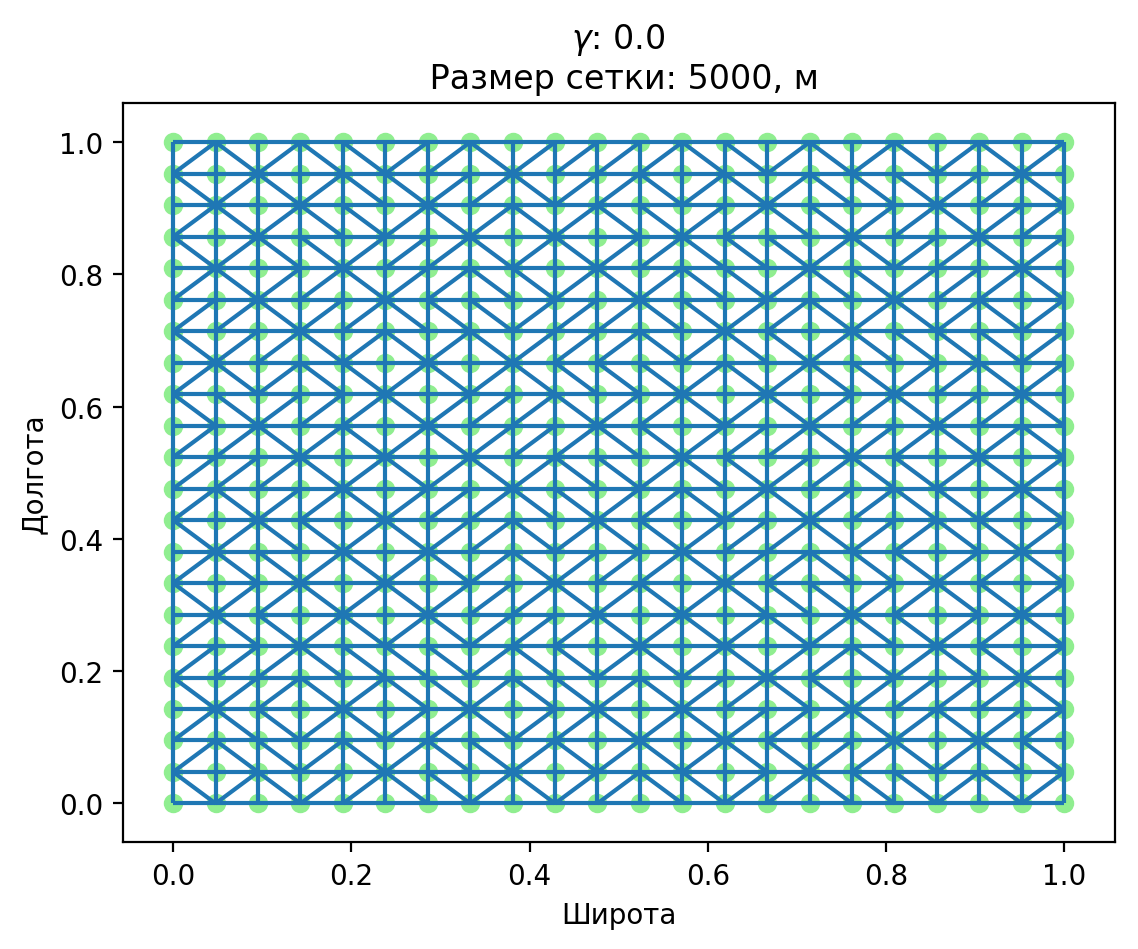
\includegraphics[width=0.5\textwidth]{images/app1_1.png}
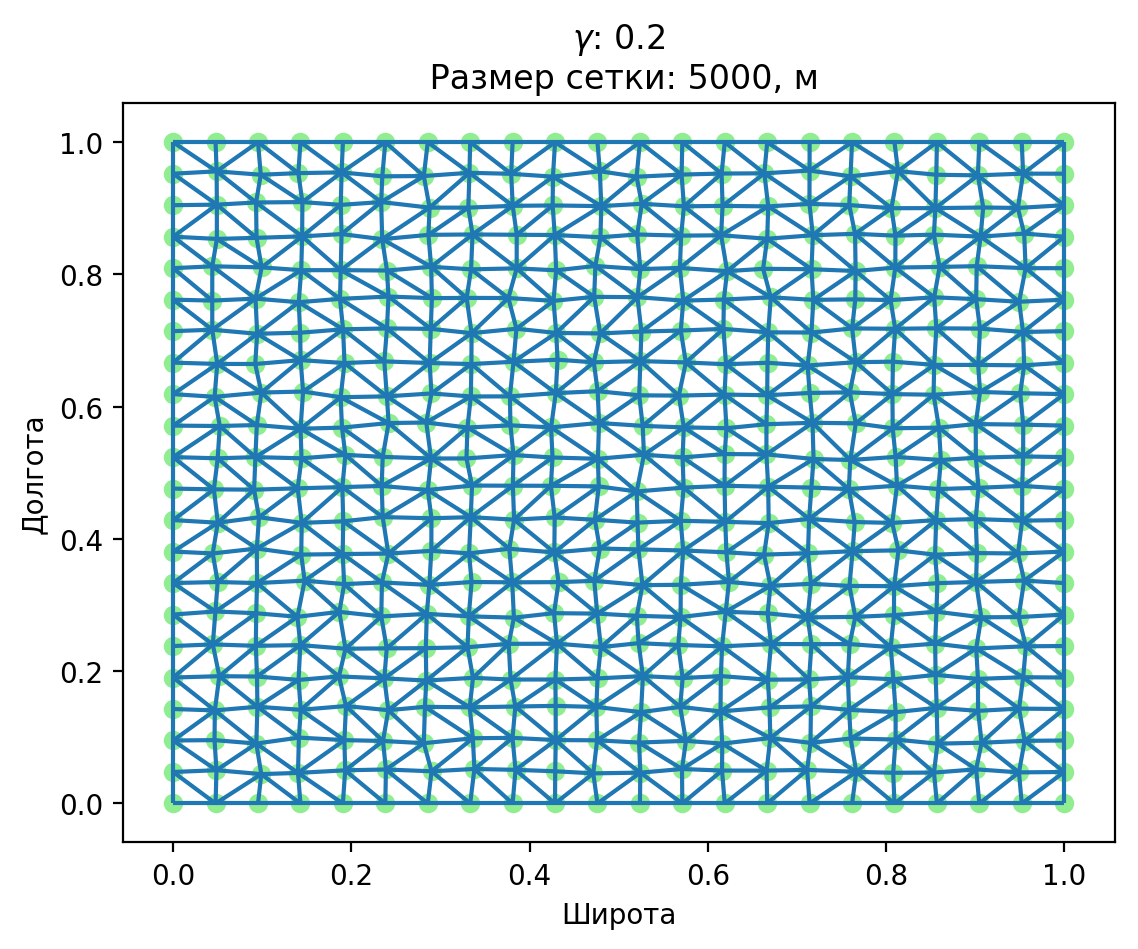
\includegraphics[width=0.5\textwidth]{images/app1_2.png}
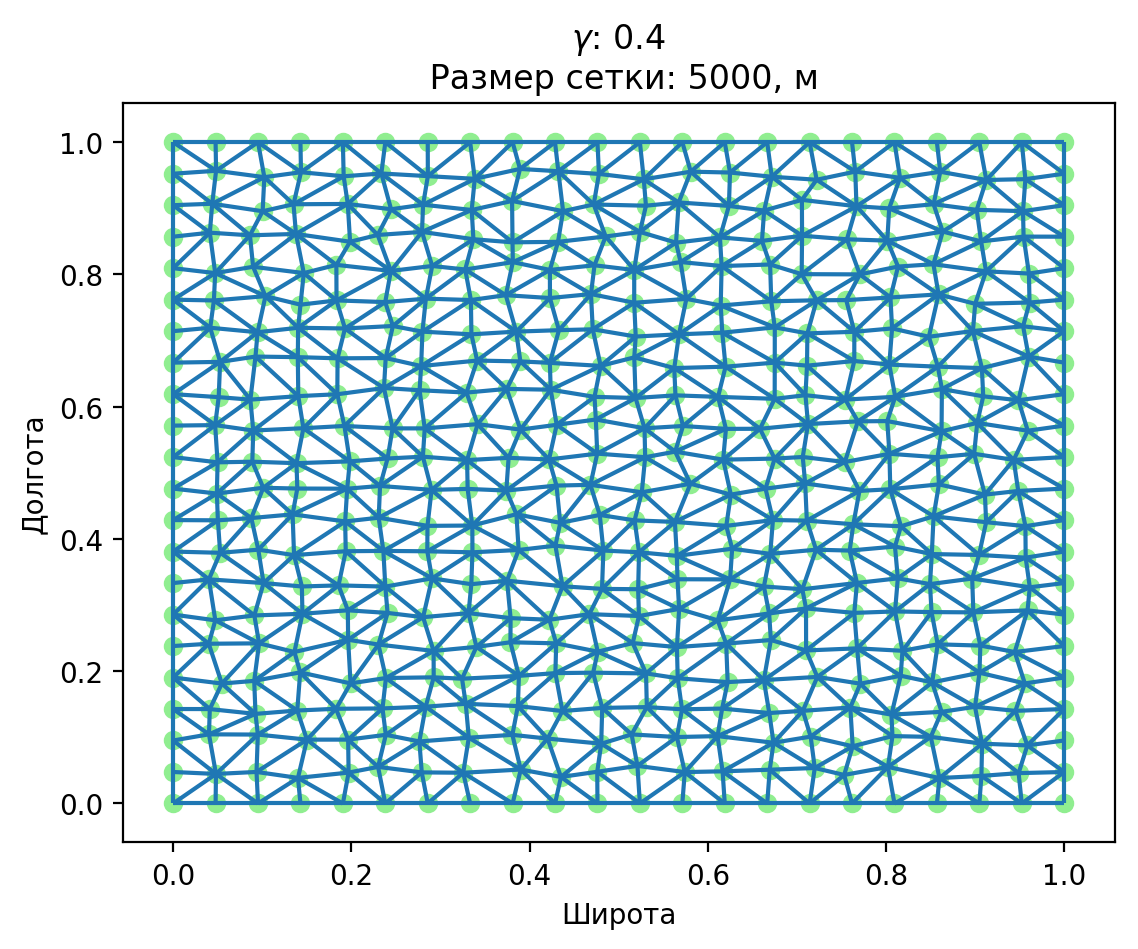
\includegraphics[width=0.5\textwidth]{images/app1_3.png}
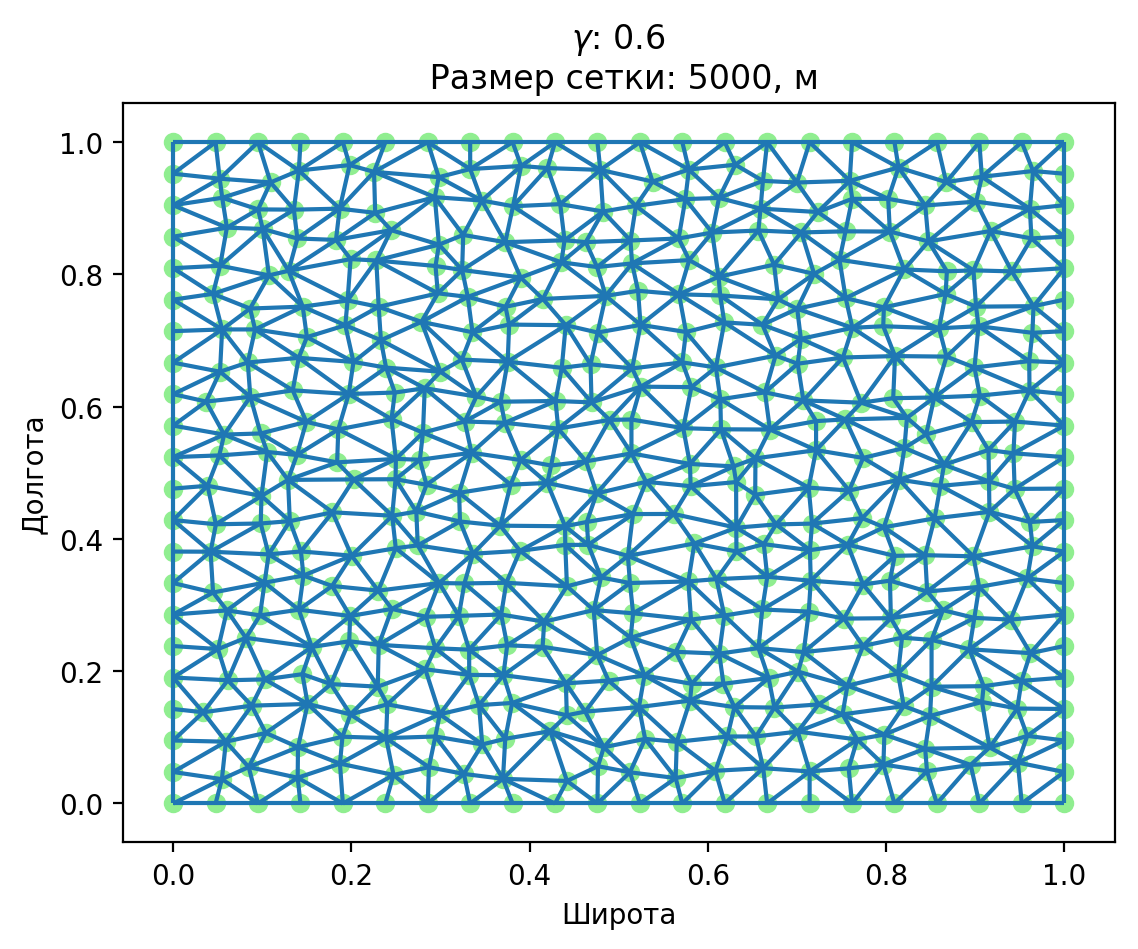
\includegraphics[width=0.5\textwidth]{images/app1_4.png}
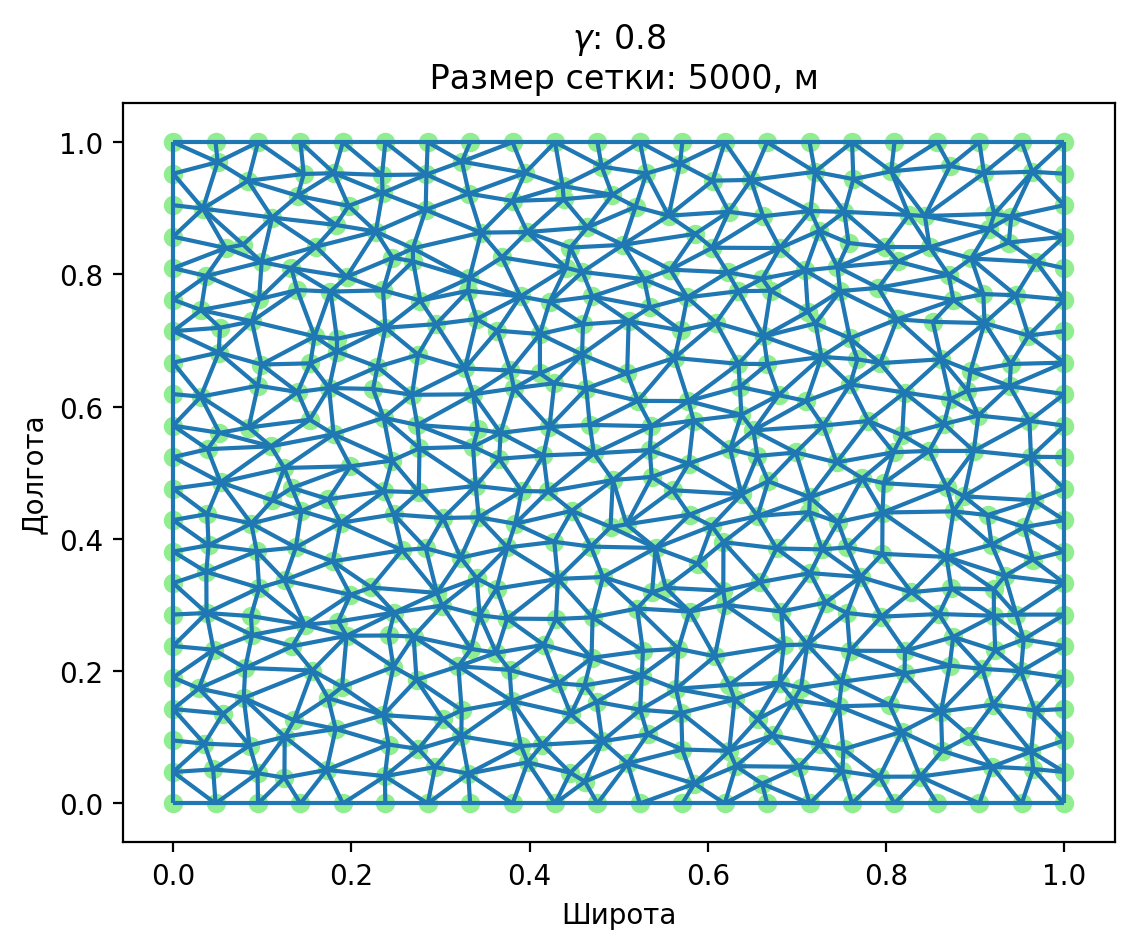
\includegraphics[width=0.5\textwidth]{images/app1_5.png}
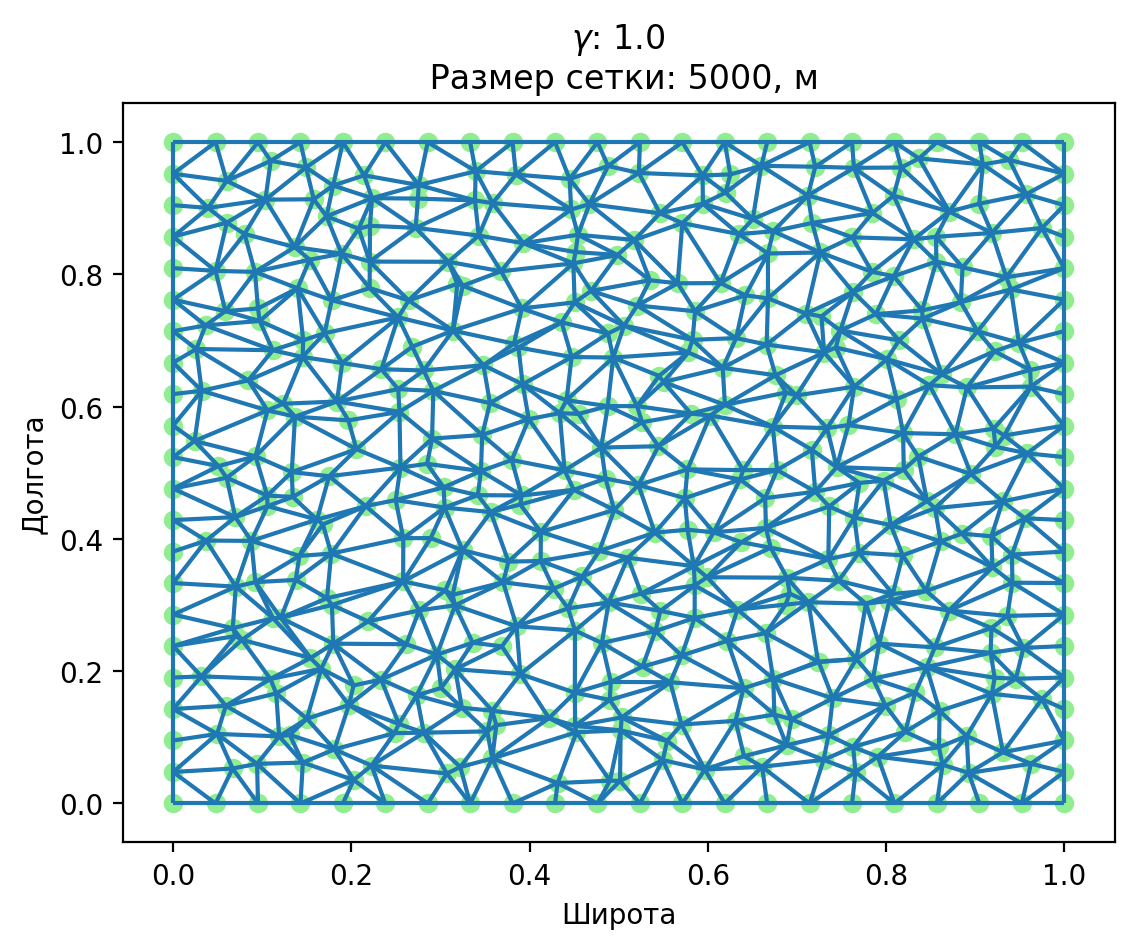
\includegraphics[width=0.5\textwidth]{images/app1_6.png}
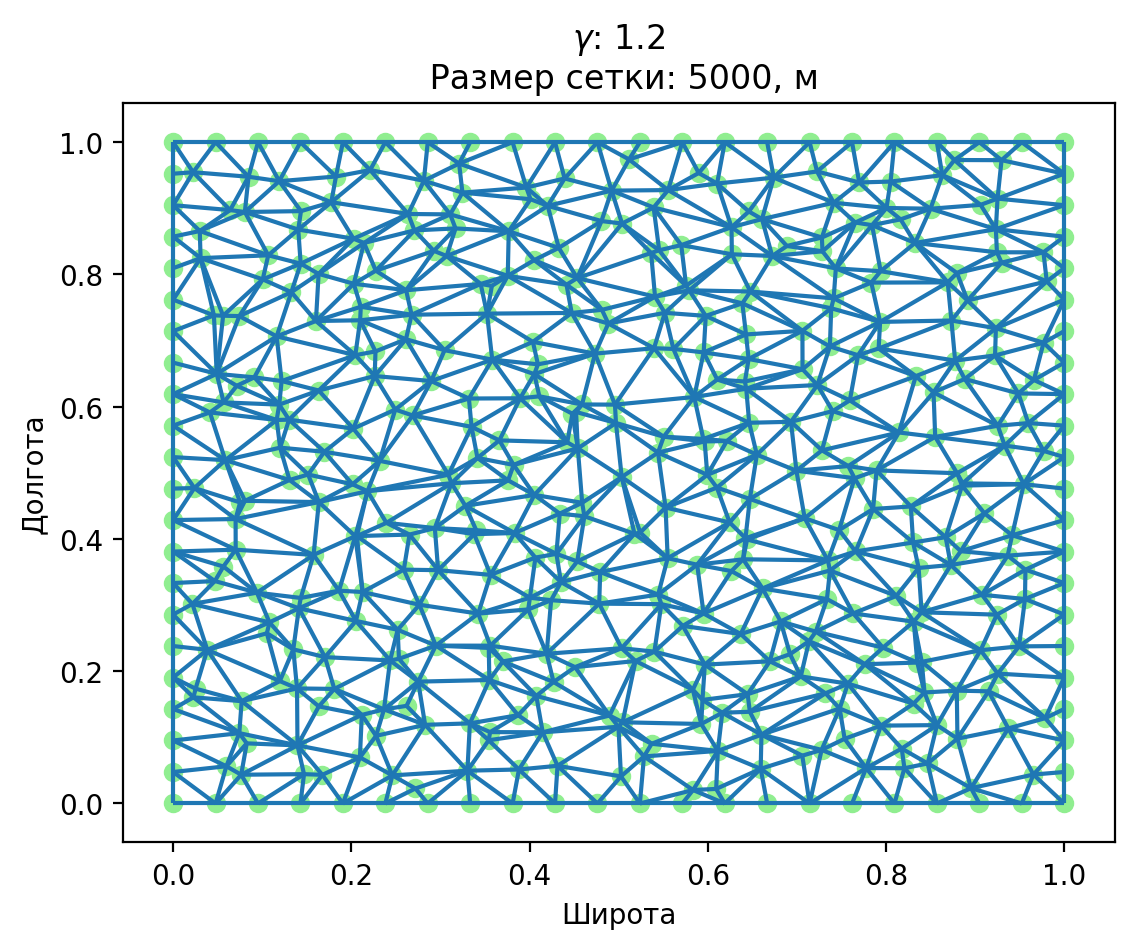
\includegraphics[width=0.5\textwidth]{images/app1_7.png}
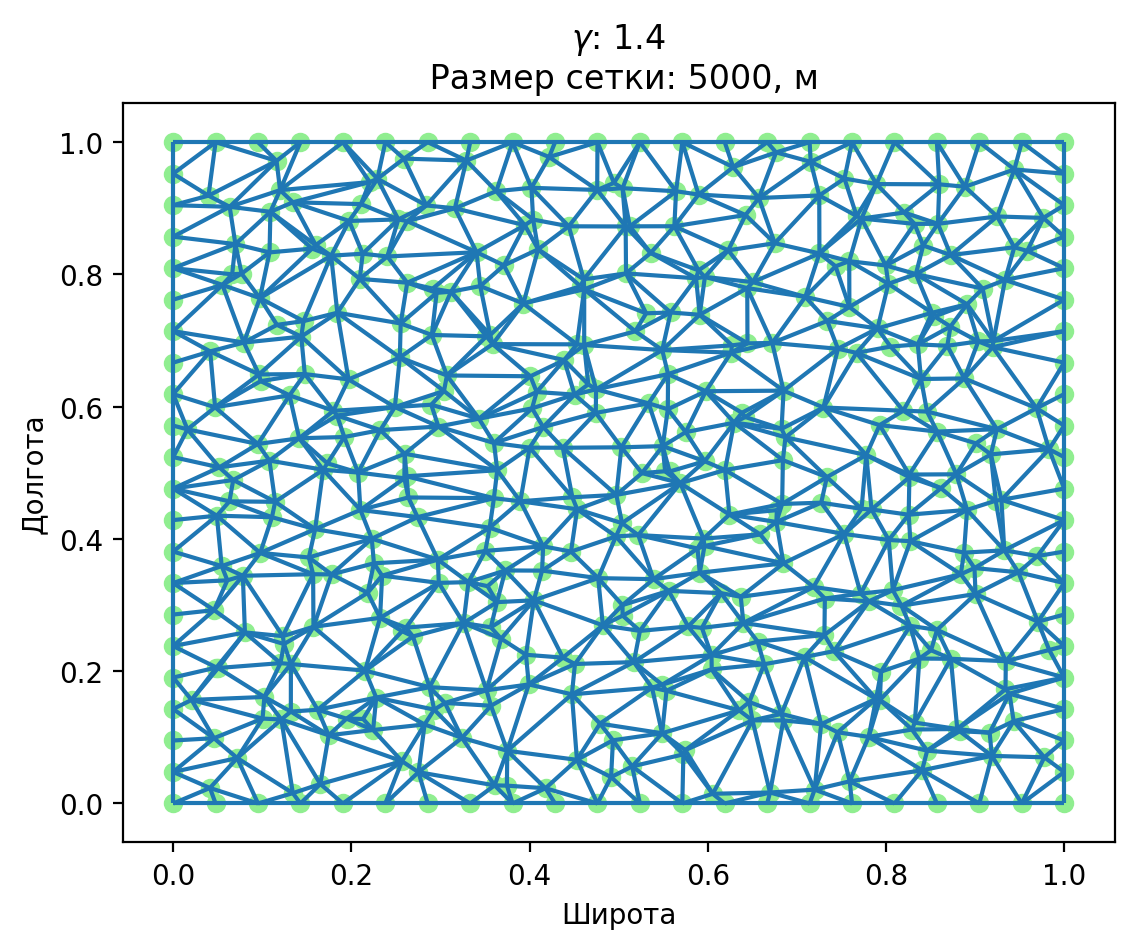
\includegraphics[width=0.5\textwidth]{images/app1_8.png}
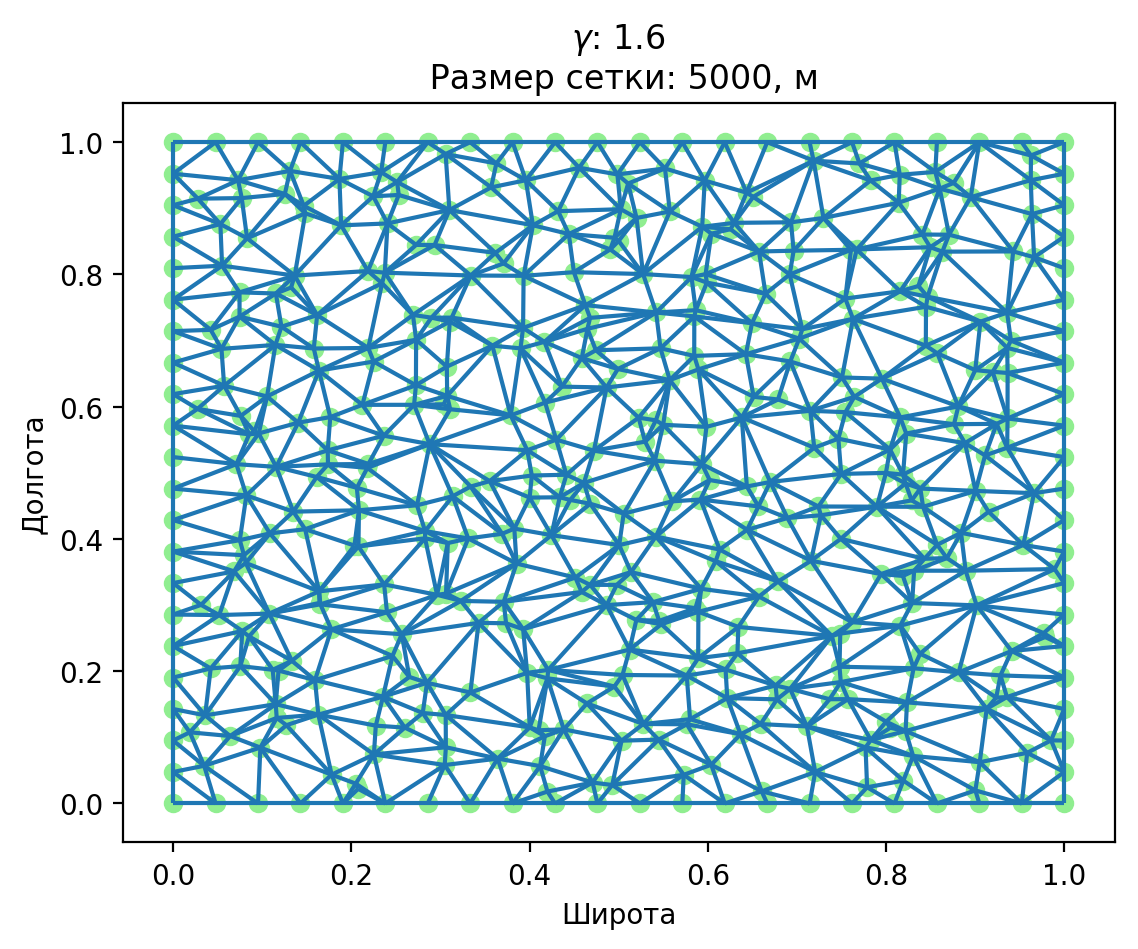
\includegraphics[width=0.5\textwidth]{images/app1_9.png}
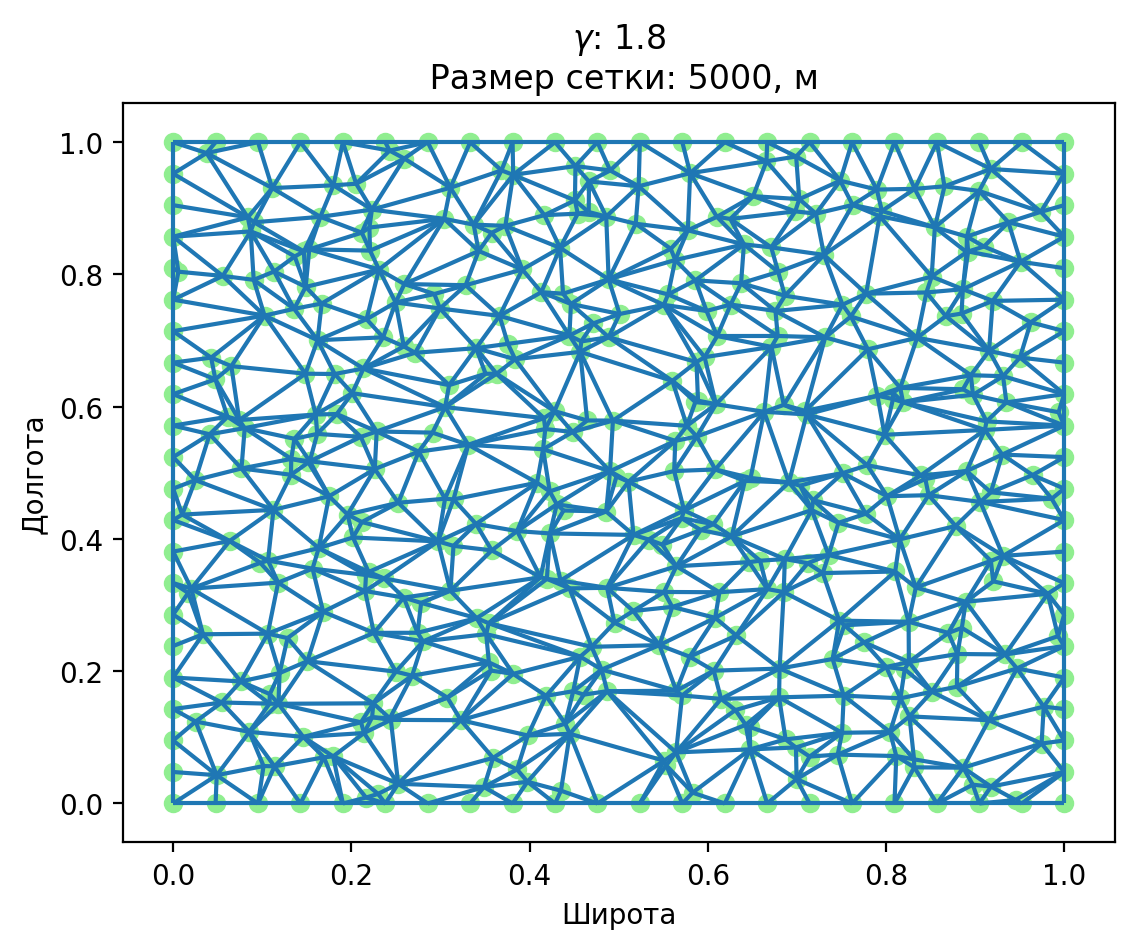
\includegraphics[width=0.5\textwidth]{images/app1_10.png}
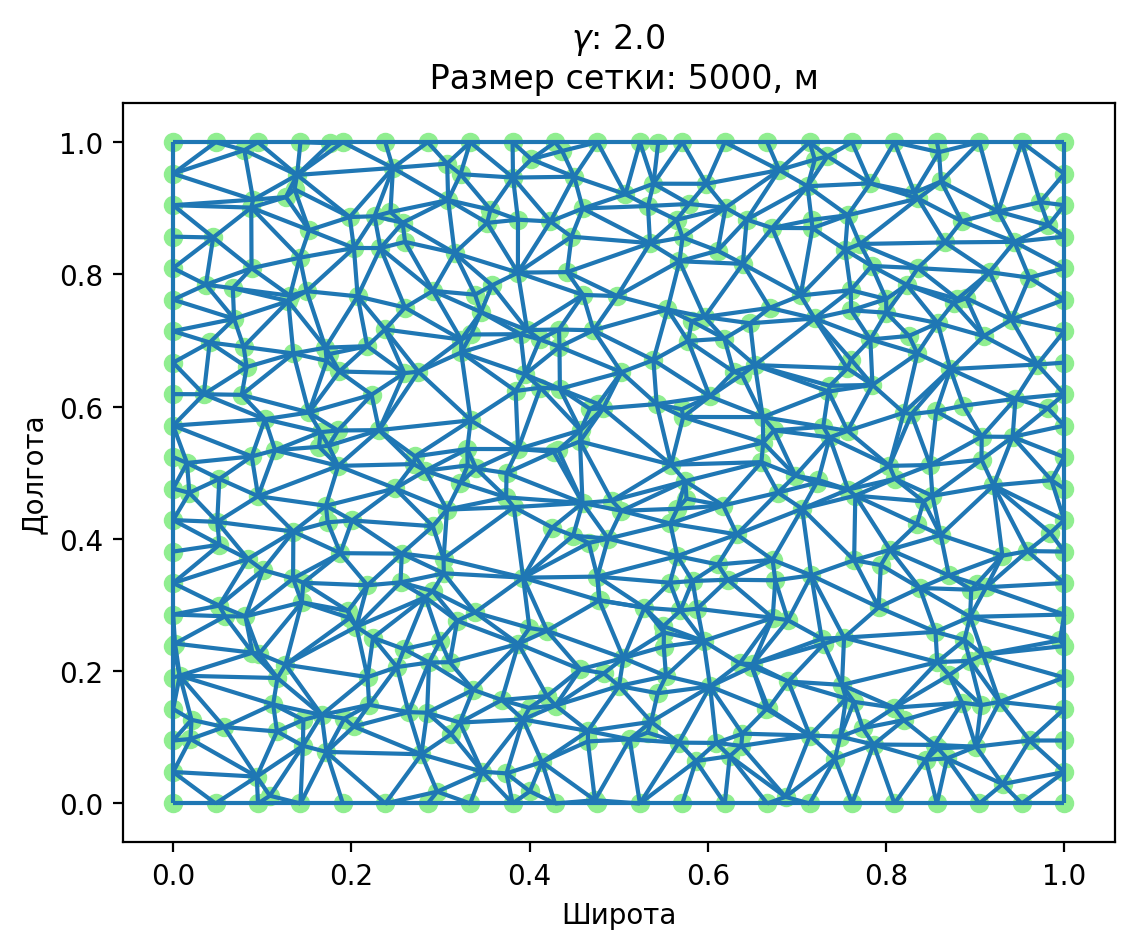
\includegraphics[width=0.5\textwidth]{images/app1_11.png}